Pour chacune des séries statistiques suivantes, donner quand c'est possible : le minimum, le premier quartile, la médiane, la moyenne et l'écart-type.

\begin{questions}
	\question[2] $12; 14 ; 2 ;  15 ; 5 ; 7 ; 8 ; 16 ; 15; 10 ; 8 ; 9 ; 14 ; 2$
	
	\fillwithdottedlines{5cm}
	
%	\question[2] $50; 80 ; 110 ; 103 ; 105 ; 107 ; 109 ; 130$
%	
%	\fillwithdottedlines{5cm}
	
	
	\question[2] $18; 17 ; 16 ; 16 ; 12 ; 12 ; 12 ; 11 ; 10 ; 9 ; 9 ; 7$
	
	\fillwithdottedlines{5cm}
	

	
	\question[2] 
	\begin{tabular}{|@{\ \ }c@{\ \ }|@{\ \ }c@{\ \ }|@{\ \ }c@{\ \ }|@{\ \ }c@{\ \ }|@{\ \ }c@{\ \ }|@{\ \ }c@{\ \ }|@{\ \ }c@{\ \ }|@{\ \ }c@{\ \ }|@{\ \ }c@{\ \ }|@{\ \ }c@{\ \ }|@{\ \ }c@{\ \ }|}
		\hline
		10 & 121 & 2 & 15 & 25 & 32 & 7 & 25 & 12 & 134 & 78 \\ \hline
		10 & 4   & 5 & 8  & 7  & 3  & 5 & 8  & 10 & 12  & 15 \\ \hline
	\end{tabular}
	
	\fillwithdottedlines{5cm}
	
	\newpage
	
	\question[2] 
	
	\begin{tabular}{|@{\ \ }c@{\ \ }|@{\ \ }c@{\ \ }|@{\ \ }c@{\ \ }|@{\ \ }c@{\ \ }|@{\ \ }c@{\ \ }|@{\ \ }c@{\ \ }|@{\ \ }c@{\ \ }|@{\ \ }c@{\ \ }|@{\ \ }c@{\ \ }|@{\ \ }c@{\ \ }|@{\ \ }c@{\ \ }|}
		\hline
		Valeur   & 22 & 25 & 27 & 29 & 121 & 124 & 125 & 127 & 128 & 129 \\ \hline
		Effectif & 1 & 2 & 1 & 4 & 8  & 14 & 10 & 8  & 5  & 2  \\ \hline
	\end{tabular}
	
	\fillwithdottedlines{5cm}
	
	\question[2] 
	
	\begin{center}
		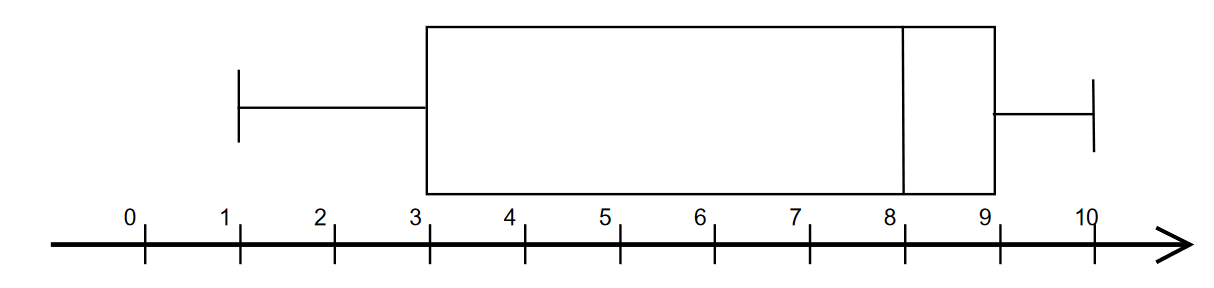
\includegraphics[scale=0.3]{boite1}
	\end{center} 

	\fillwithdottedlines{5cm}
	
\end{questions}